\documentclass[tikz,border=8pt]{standalone}
% Shared look for every TikZ diagram. Load with % Shared look for every TikZ diagram. Load with % Shared look for every TikZ diagram. Load with \input{../../tools/tikz-style.tex}
\usepackage[T1]{fontenc}
\usepackage{lmodern}
\renewcommand{\sfdefault}{lmr}  % diagrams use the same serif as the text
\usetikzlibrary{arrows.meta, positioning, shapes.geometric, calc, fit, backgrounds}
\definecolor{cblue}{HTML}{4C78A8}
\definecolor{corange}{HTML}{F58518}
\definecolor{cgreen}{HTML}{54A24B}
\definecolor{cred}{HTML}{E45756}
\definecolor{cpurple}{HTML}{B279A2}
\definecolor{cgrey}{HTML}{6B6B6B}
\tikzset{
  every picture/.style={font=\sffamily, line width=1.2pt},
  box/.style={draw=#1, fill=#1!12, rounded corners=4pt, align=center, inner sep=7pt, minimum height=1.1cm},
  box/.default=cgrey,
  arrow/.style={-{Stealth[length=3mm]}, draw=cgrey, line width=1.4pt},
  title/.style={font=\sffamily\bfseries\Large},
  note/.style={font=\sffamily\small, text=cgrey, align=center},
}
\AtBeginDocument{\hyphenpenalty=10000 \exhyphenpenalty=10000}

\usepackage[T1]{fontenc}
\usepackage{lmodern}
\renewcommand{\sfdefault}{lmr}  % diagrams use the same serif as the text
\usetikzlibrary{arrows.meta, positioning, shapes.geometric, calc, fit, backgrounds}
\definecolor{cblue}{HTML}{4C78A8}
\definecolor{corange}{HTML}{F58518}
\definecolor{cgreen}{HTML}{54A24B}
\definecolor{cred}{HTML}{E45756}
\definecolor{cpurple}{HTML}{B279A2}
\definecolor{cgrey}{HTML}{6B6B6B}
\tikzset{
  every picture/.style={font=\sffamily, line width=1.2pt},
  box/.style={draw=#1, fill=#1!12, rounded corners=4pt, align=center, inner sep=7pt, minimum height=1.1cm},
  box/.default=cgrey,
  arrow/.style={-{Stealth[length=3mm]}, draw=cgrey, line width=1.4pt},
  title/.style={font=\sffamily\bfseries\Large},
  note/.style={font=\sffamily\small, text=cgrey, align=center},
}
\AtBeginDocument{\hyphenpenalty=10000 \exhyphenpenalty=10000}

\usepackage[T1]{fontenc}
\usepackage{lmodern}
\renewcommand{\sfdefault}{lmr}  % diagrams use the same serif as the text
\usetikzlibrary{arrows.meta, positioning, shapes.geometric, calc, fit, backgrounds}
\definecolor{cblue}{HTML}{4C78A8}
\definecolor{corange}{HTML}{F58518}
\definecolor{cgreen}{HTML}{54A24B}
\definecolor{cred}{HTML}{E45756}
\definecolor{cpurple}{HTML}{B279A2}
\definecolor{cgrey}{HTML}{6B6B6B}
\tikzset{
  every picture/.style={font=\sffamily, line width=1.2pt},
  box/.style={draw=#1, fill=#1!12, rounded corners=4pt, align=center, inner sep=7pt, minimum height=1.1cm},
  box/.default=cgrey,
  arrow/.style={-{Stealth[length=3mm]}, draw=cgrey, line width=1.4pt},
  title/.style={font=\sffamily\bfseries\Large},
  note/.style={font=\sffamily\small, text=cgrey, align=center},
}
\AtBeginDocument{\hyphenpenalty=10000 \exhyphenpenalty=10000}

% one column of cells: \col{x}{y}{name}{colour}{v1,v2,...}
\newcommand{\col}[5]{
  \node[font=\sffamily\bfseries\small, text=#4] at (#1,#2+0.6) {#3};
  \foreach \v [count=\i] in {#5} {
    \node[draw=#4, fill=#4!10, minimum width=2.3cm, minimum height=0.75cm] at (#1,#2-0.75*\i+0.35) {\v};
  }
}
\begin{document}
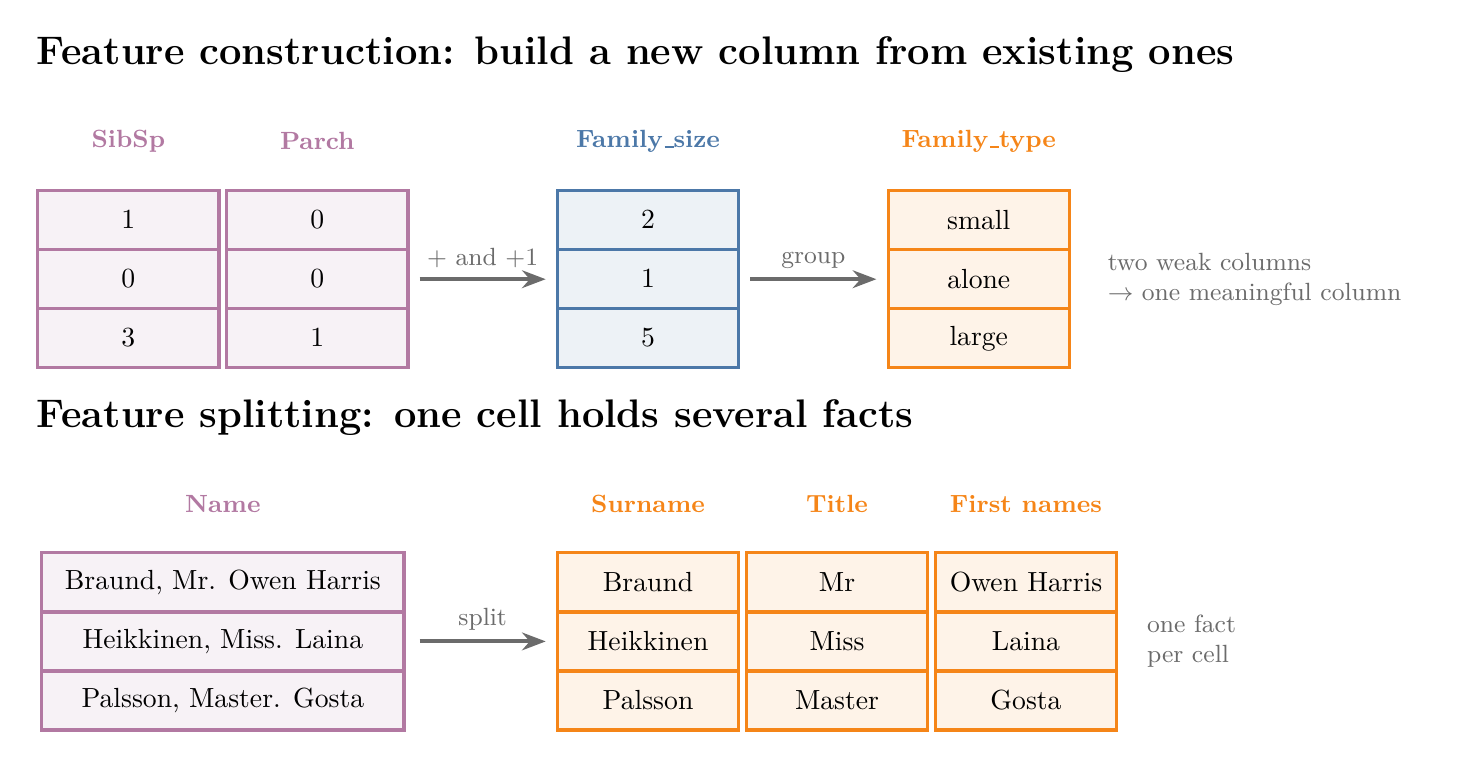
\begin{tikzpicture}
  % construction
  \node[title, anchor=west] at (-1.3,1.7) {Feature construction: build a new column from existing ones};
  \col{0}{0}{SibSp}{cpurple}{1, 0, 3}
  \col{2.4}{0}{Parch}{cpurple}{0, 0, 1}
  \draw[arrow] (3.7,-1.15) -- node[above, note] {$+$ and $+1$} (5.3,-1.15);
  \col{6.6}{0}{Family\_size}{cblue}{2, 1, 5}
  \draw[arrow] (7.9,-1.15) -- node[above, note] {group} (9.5,-1.15);
  \col{10.8}{0}{Family\_type}{corange}{small, alone, large}
  \node[note, anchor=west, text width=4.2cm, align=left] at (12.3,-1.15) {two weak columns\\ $\rightarrow$ one meaningful column};
  % splitting
  \begin{scope}[yshift=-4.6cm]
  \node[title, anchor=west] at (-1.3,1.7) {Feature splitting: one cell holds several facts};
  \node[font=\sffamily\bfseries\small, text=cpurple] at (1.2,0.6) {Name};
  \node[draw=cpurple, fill=cpurple!10, minimum width=4.6cm, minimum height=0.75cm] at (1.2,-0.4) {Braund, Mr. Owen Harris};
  \node[draw=cpurple, fill=cpurple!10, minimum width=4.6cm, minimum height=0.75cm] at (1.2,-1.15) {Heikkinen, Miss. Laina};
  \node[draw=cpurple, fill=cpurple!10, minimum width=4.6cm, minimum height=0.75cm] at (1.2,-1.9) {Palsson, Master. Gosta};
  \draw[arrow] (3.7,-1.15) -- node[above, note] {split} (5.3,-1.15);
  \col{6.6}{0}{Surname}{corange}{Braund, Heikkinen, Palsson}
  \col{9.0}{0}{Title}{corange}{Mr, Miss, Master}
  \col{11.4}{0}{First names}{corange}{Owen Harris, Laina, Gosta}
  \node[note, anchor=west, text width=2.8cm, align=left] at (12.8,-1.15) {one fact\\ per cell};
  \end{scope}
\end{tikzpicture}
\end{document}
